\documentclass[14pt]{article}
%\usepackage[cp1251]{inputenc}
\usepackage[english,russian]{babel}
\usepackage{amssymb,latexsym,amsmath,euscript,amsfonts,amsthm}
\usepackage{color}
\linespread{1.5}

\usepackage{fontspec}
\usepackage{polyglossia}
\setdefaultlanguage{russian}
\setmainfont[Mapping=tex-text]{CMU Serif}
\usepackage[font=small]{caption}
%\usepackage{subcaption}
%\usepackage{hyperref}
%\usepackage{sidecap}
\usepackage{float} %for fig position
\usepackage{graphicx}
\graphicspath{{pictures/}}
\DeclareGraphicsExtensions{.pdf,.png,.jpg}
\usepackage[left=30mm, top=20mm, right=30mm, bottom=20mm, nohead, footskip=10mm]{geometry}
%\setlength{\textfloatsep}{10pt plus 1.0pt minus 2.0pt}

\title{Курсовая работа}
\author{Соколова Ирина}

\newtheorem{theorem}{Теорема}
\newtheorem{lemma}{Лемма}
%\newtheorem*{corollary}{Следствие}[chapter]
\newtheorem{definition}{Определение}
%\newtheorem*{conjecture}{Гипотеза}
%\newtheorem*{example}{Пример}
%\newtheorem*{remark}{Замечание}[chapter]
%\newtheorem*{criteria}{Критерий}

\newcommand{\RomanNumeralCaps}[1]
    {\MakeUppercase{\romannumeral #1}}

%\newcounter{exercise}
%\newenvironment{exercise}{\refstepcounter{exercise}\smallskip\noindent\textbf{Упражнение~\theexercise.}}{}
%\numberwithin{exercise}

%\newenvironment{demo}{\noindent\textsl{Доказательство. }}{ $\square$ \medskip}

\begin{document}
\pagestyle{plain}
\makeatletter

\begin{titlepage}
\begin{center}
\textbf{Правительство Российской Федерации}\\
\textbf{Федеральное государственное автономное образовательное}\\
\textbf{учреждение высшего профессионального образования}\\
\textbf{"Национальный исследовательский университет}\\
\textbf{Высшая школа экономики"}\\
\textbf{Нижний Новгород}\\
\bigskip
\bigskip
\bigskip
\bigskip
\bigskip
\bigskip
\bigskip
\bigskip
\bigskip
\bigskip
\bigskip
\bigskip
\bigskip
\bigskip
\bigskip
\textbf{Факультет Информатики,  Математики и Компьютерных Наук}\\
\textbf{Программа подготовки бакалавров:}\\
\normalsize{ Фундаментальная математика}\\
\normalsize{ 2019-2020 учебный год}\\
\bigskip
\bigskip
\bigskip
\bigskip
\bigskip
\footnotesize\uppercase{курсовая работа}\\
\bigskip
\textbf{\large{О расположениях кубики и пары коник в вещественной}}\\
\textbf{\large{проективной плоскости}}\\
\bigskip
\bigskip
\bigskip
\bigskip
\bigskip
\end{center}
\bigskip
\bigskip
\bigskip
\begin{flushright}
\textbf{Выполнила:}
\normalsize{Соколова Ирина Максимовна}\\
\end{flushright}
\bigskip
\begin{flushleft}
\textbf{Научный руководитель:}\\
\normalsize{Кандидат физико-математических}\\
\normalsize{наук, доцент}\\
\normalsize{Полотовский Григорий Михайлович}\\
\normalsize{Подпись:}
\bigskip
\bigskip
\end{flushleft}
\vfill
\begin{center} Нижний Новгород, 2020 \end{center}
\end{titlepage}

%\tableofcontents

\newpage
\section{Введение}


        На \RomanNumeralCaps{2} Международном Конгрессе математиков в Париже в 1900 году немецким математиком Д. Гильбертом были сформулированы 23 математические проблемы, которые предстояло решить в \RomanNumeralCaps{20} веке. Одной из этих проблем, а именно шестнадцатой, является «Проблема топологии алгебраических кривых и поверхностей». Шестнадцатая проблема Гильберта разбивается на две части, первая из которых – это исследование топологии неособых алгебраических кривых на проективной плоскости $\mathbb RP^2$ и неособых алгебраических поверхностей в проективном пространстве $RP^3$. К теме шестнадцатой проблемы Гильберта примыкает задача исследования топологии вещественных алгебраических многообразий размерности $d$ в вещественном проективном пространстве $RP^q$, где $q \geqslant 3, 1 \leqslant d \leqslant (q–1)$, а также исследование вещественных алгебраических многообразий с особенностями.
\newpage
\section{Постановка задачи}

\begin{definition}
 Плоской вещественной проективной алгебраической кривой степени m называется однородный многочлен $\mathbb C_m(x_0, x_1, x_2)$ степени m с вещественными коэффициентами от трёх переменных $x_0, x_1, x_2$, рассматриваемый с точностью до ненулевого постоянного множителя.
\end{definition}

\begin{definition}
Множество $\mathbb RC_m$ точек вещественной проективной плоскости $\mathbb RP^2$ с координатами $(x_0:x_1:x_2)$, удовлетворяющими уравнению $\mathbb C_m = 0$, называется множеством вещественных точек кривой $\mathbb C_m$.
\end{definition}

\begin{definition}
Кривая $\mathbb C_m$ называется неoсобой, если частные производные многочлена $\mathbb C_m$ одновременно не равны нулю.
\end{definition}

\begin{definition}
Пусть $F$ – однородный многочлен степени $m$ от переменных $x_1, x_2, x_3$. Если выполнено равенство $F = F_1 \cdot F_2$, где $F_1, F_2$ – однородные многочлены степеней $m_1$ и $m_2$ соответственно, $1 \leqslant m_1 < m, 1 \leqslant m_2 < m$, то многочлен называется распадающимся, иначе -- нераспадающимся. Каждая из кривых $F_1 = 0$ и $F_2 = 0$ называется сомножителем кривой $F$.
\end{definition}

Каждая компонента связности множества  $\mathbb RC_m$ вещественных точек неособой кривой $\mathbb C_m$ гомеоморфна окружности. В случае четной степени эта окружность называется овалом; каждый овал делит $\mathbb RP^2$ на две области: гомеоморфную диску и гомеоморфную листу Мебиуса. В случае нечетной степени среди вещественных ветвей кроме овалов имеется ровна одна ветвь, вложенная в $\mathbb RP^2$ односторонне, она называется нечетной ветвью.

\begin{theorem}[Теорема Харнака]
Пусть $N$ -- число вещественых ветвей кривой $\mathbb C_m$. Тогда выполняется следующее неравенство $N \leqslant (m-1) \cdot (m – 2)/2 + 1$, и эта оценка точна для любого $m$.
\end{theorem}

\begin{definition}
Кривые с максимально возможным по теореме Харнака числом ветвей называются М-кривыми.
\end{definition}

В этой работе мы будем рассматривать кривые степени 7, распадающиеся на две коники (обозначим их $C_2$ и $C_2^*$) и кубику (обозначим $C_3$) с выполнением следующих условий:

\begin{enumerate}
\item $C_3$, $C_2$, $C_2^*$ являются \textit{М}-кривыми.
\item Кривые, указанные в п. 1, попарно пересекаются без касания в максимально возможном (по теореме Безу) числе вещественных точек. Таким образом, $C_2$ и $C_3$ пересекаются в шести точках, $C_2^*$ и $C_3$ пересекаются в шести точках, $C_2$ и $C_2*$ – в  четырёх точках. 
\item Ни через какую точку не проходят сразу три кривые из п. 1.
\item Для каждой из коник $C_2$, $C_2^*$ пять общих точек нечетной ветви кубики и коники лежат на одной из четырех внешних (то есть лежащих вне другой коники) дуг, на которые эта коника делится точками пересечения со второй коникой, а шестая точка пересечения лежит на одной из двух внутренних (то есть лежащих внутри другой коники) дуг.
\item Сначала нечетная ветвь пять раз пересекает первую конику, затем - один раз вторую конику, затем - первую конику один раз  и после пересекает вторую конику пять раз (рисунок \ref{fig:model_1-5}).
\end{enumerate}

\begin{figure}[H]
\center{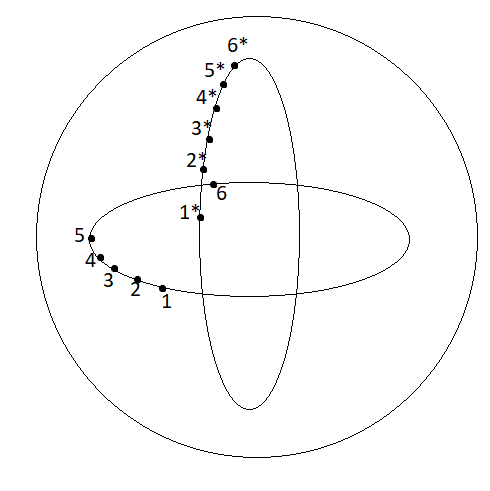
\includegraphics[scale=0.55]{model_1-5.png}}
\caption{Модель}
\label{fig:model_1-5}
\end{figure}

Зачача состоит в топологической классификации кривых такого вида в проективной плоскости. В этой работе мы выполним первый этап решения этой задачи: найдём список топологических моделей таких кривых, не противоречащих топологическим следствиям теоремы Безу.

\begin{definition}
Назовём моделью расположения типа $1-5$ (в дальнейшем – просто модель) набор четырёх топологических окружностей, ровно одна из которых вложена в $\mathbb RP^2$ односторонне и которая вместе с двумя из трёх остальных окружностей ведет себя с точки зрения числа и расположения общих точек, как описано в пунктах $1-5$; четвёртая окружность не пересекается с первыми тремя.
\end{definition}

Будем учитывать известные сведения о взаимных расположениях \textit{М}-кубики и неособой коники: имеются ровно три таких расположения, в которых нечётная ветвь кубики пересекает конику в шести вещественных точках (рисунок \ref{fig:ovals_and_loc_of_odd_brunch}).

\begin{figure}[H]
\center{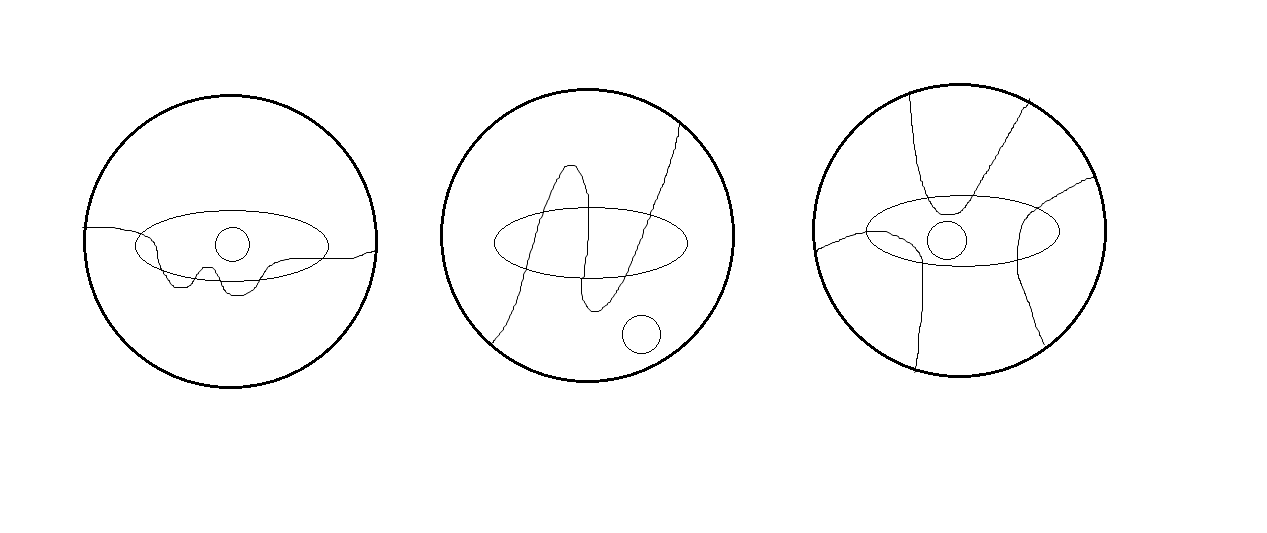
\includegraphics[scale=0.55]{ovals_and_loc_of_odd_brunch.png}}
\caption{Расположения нечетной ветви а) б) с)}
\label{fig:curves_with_ovals}
\end{figure}

Третий случай пересечения коники нечетной ветвбью в шести точках рассматриать не будем.

Пусть $\mathbb RC_2$ – «горизонтальный» овал, $\mathbb RC_2^*$ – «вертикальный» овал. Рассмотрим все возможные способы пересечения нечетной ветви с внешней дугой одной из коник (аналогичные возможные случаи пересечения нечетной ветви будут и с внешней дугой другой коники). Не нарушая общности, будем всегда рассматривать начало пересечения нечетной ветви с кониками на левой внешней дуге $\mathbb RC_2$. 

Двигаясь по направлению часовой стрелки, будем записывать номера точек пересечения нечетной ветви с левой внешней дугой $\mathbb RC_2$. При рассмотрении всевозможных пересечений нечетной ветви с $\mathbb RC_2$ в пяти точках мы получим всевозможные перестановки порядка 5 (например на рисунке \ref{fig:model_1-5} это перестановка $(1,2,3,4,5)$ ).
\\
Необходимо перебрать все перестановки степени 5. Большая часть перестановок запретится либо в силу того, что нечётная ветвь М-кривой не может иметь самопересечений(рисунок \ref{fig:two_bad_ex} а), либо теоремой Безу (рисунок \ref{fig:two_bad_ex} б).

\begin{figure}[H]
        \center{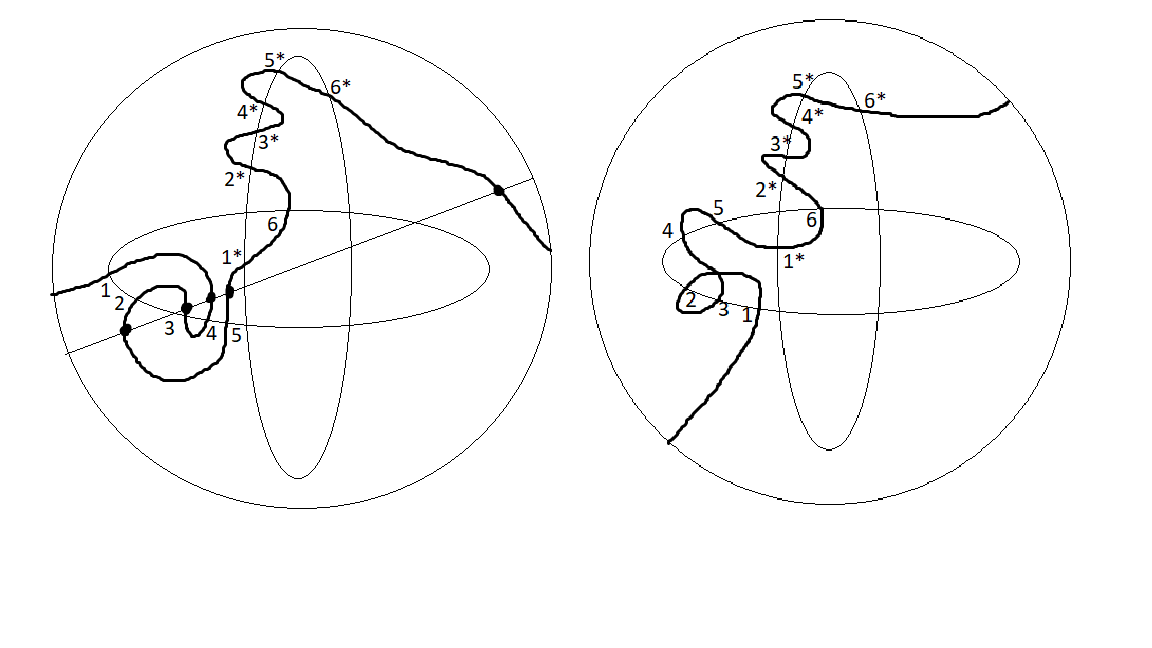
\includegraphics[scale=0.45]{two_bad_ex.png}}
        \caption{a) б)}
    \label{fig:two_bad_ex}
\end{figure}

Непосредственным перебором мы получим следующие возможные перестановки:\\
(12345), (32145) – случай пересечения нечетной ветвью коники образом, показанным на рисунке \ref{fig:curves_with_ovals} а)\\ 
(54123), (54321) – случай пересечения нечетной ветвью коники образом, показанным на рисунке \ref{fig:curves_with_ovals} б)\\ 
\\
Существует два возможных расположения в $\mathbb RP^2$ двух неособых коник с четырьмя общими точками (рисунок ниже).
\\

\begin{figure}[H]
\center{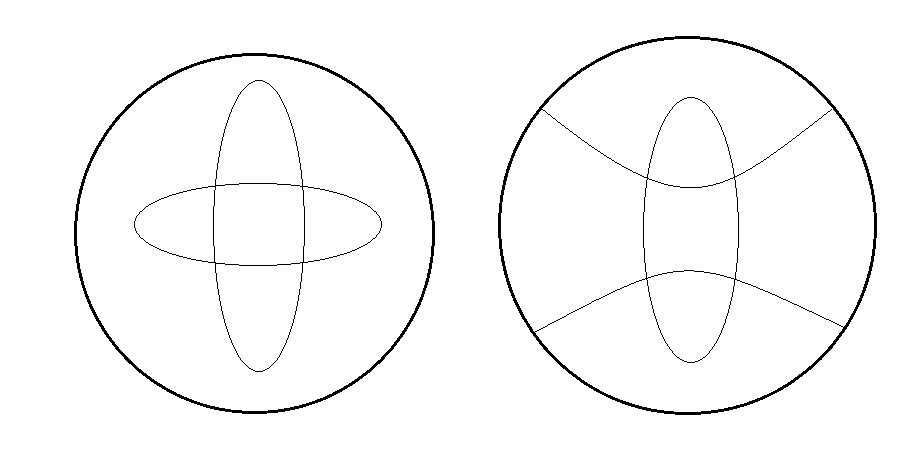
\includegraphics[scale=0.45]{intersection_of_ovals.png}}
\caption{}
\label{fig:intersection_of_ovals}
\end{figure}

Но в случае, который представлен на рисунке \ref{fig:intersection_of_ovals} справа, расположение нечетной ветви будет противоречить пункту 5 - при соблюдении условий 1-4 не будет соблюдаться условие 5 (рисунок \ref{fig:prohibit_3_case_loc_odd_brunch}),  поэтому мы будем рассматривать только первый случай .

\begin{figure}[H]
\center{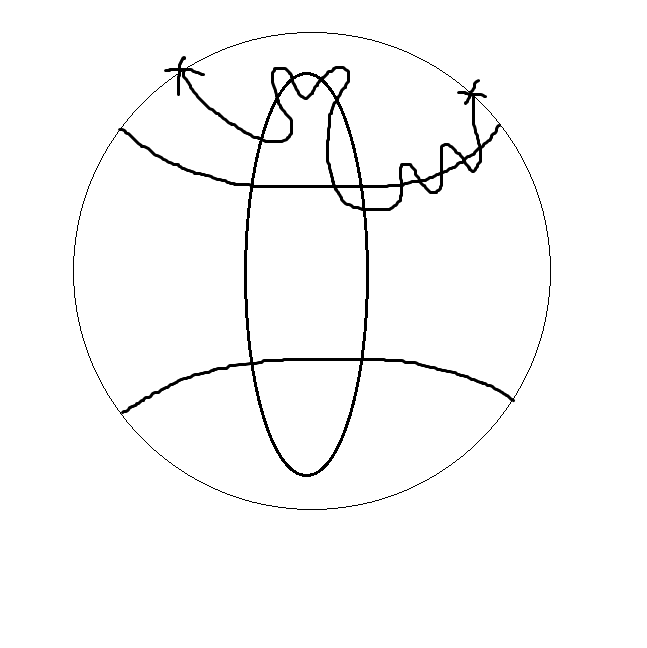
\includegraphics[scale=0.55]{prohibit_3_case_loc_odd_brunch.png}}
\caption{}
\label{fig:prohibit_3_case_loc_odd_brunch}
\end{figure}


Проиллюстрируем случаи пересечения нечетной ветви с кониками, соответствующие оставшимся подстановкам. Всего получится $4 \cdot 4 = 16$ иллюстраций, но некоторые из них дают гомеоморфные картинки, попарно негомеоморфных получилось 11. 
После соблюдения всех вышеперечисленных условий мы получим следующие возможные расположения нашей М-кривой седьмой степени, без учета возможного расположения овала:

\begin{figure}[H]
\center{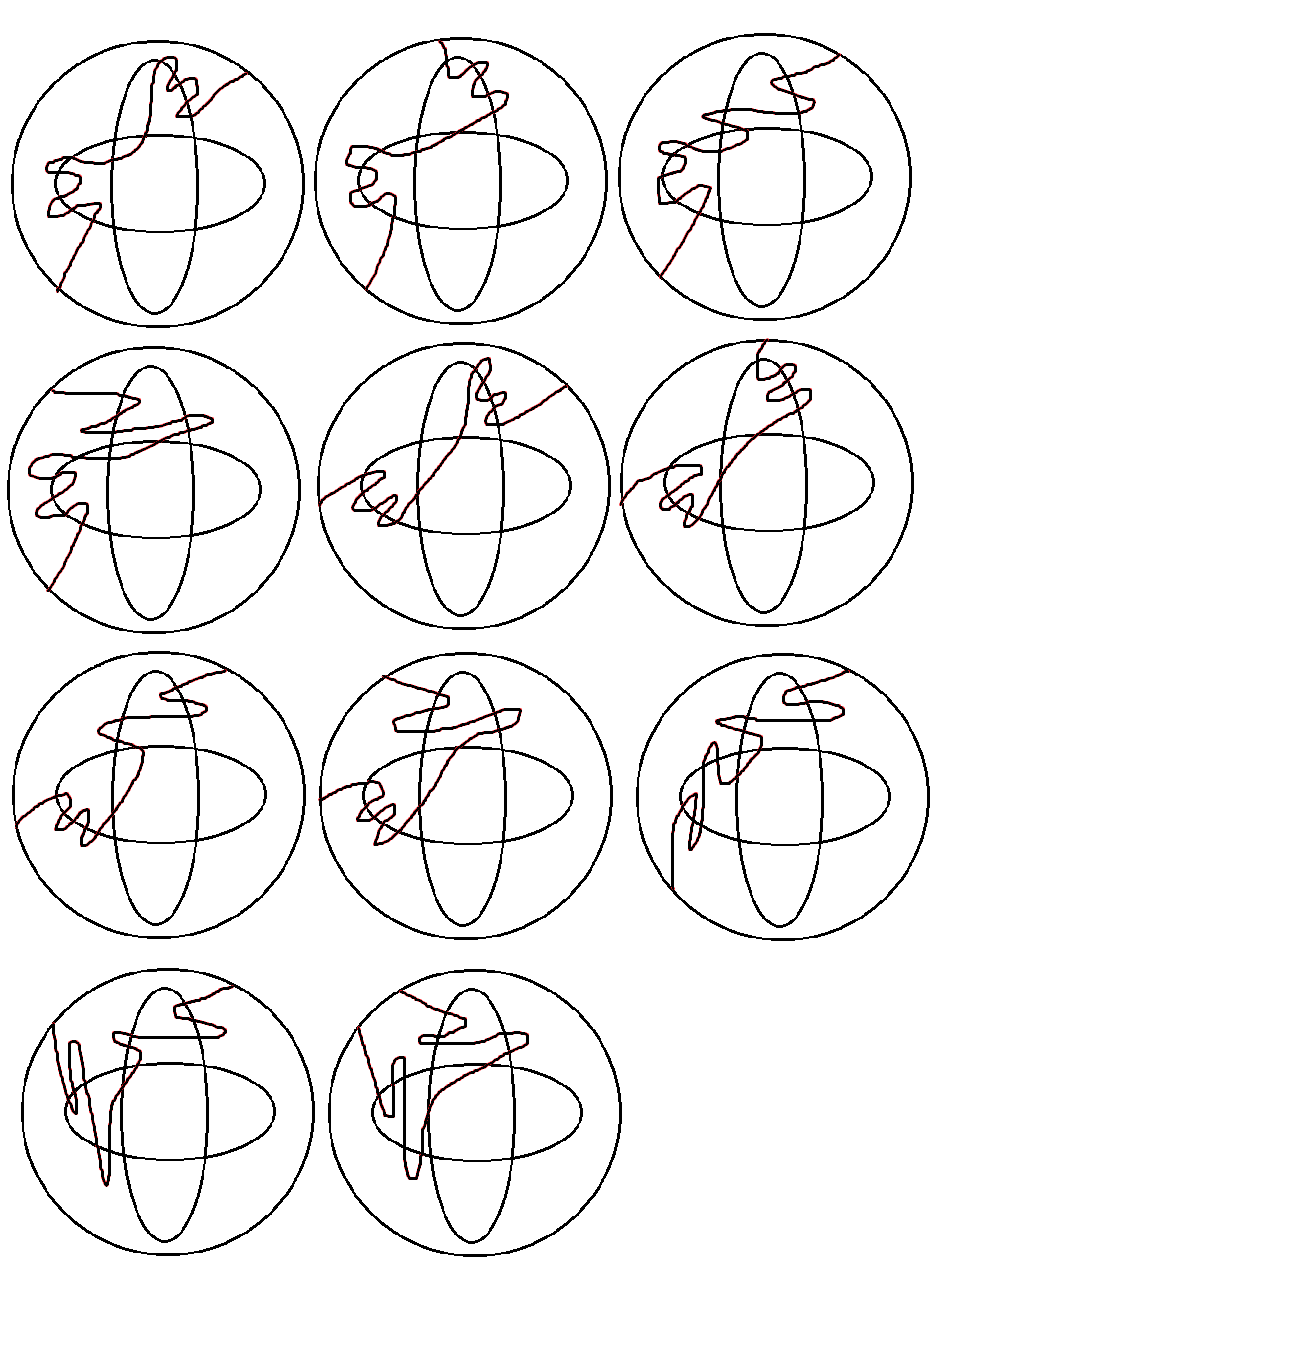
\includegraphics[scale=0.75]{curves_without_ovals.png}}
\caption{Модели без овалов}
\label{fig:curves_without_ovals}
\end{figure}
Допустимые для расположения овала кубики компоненты дополнения $\mathbb RP^2$ к объединению коники и кубики показаны на рисунке \ref{fig:ovals_and_loc_of_odd_brunch}.

\begin{figure}[H]
\center{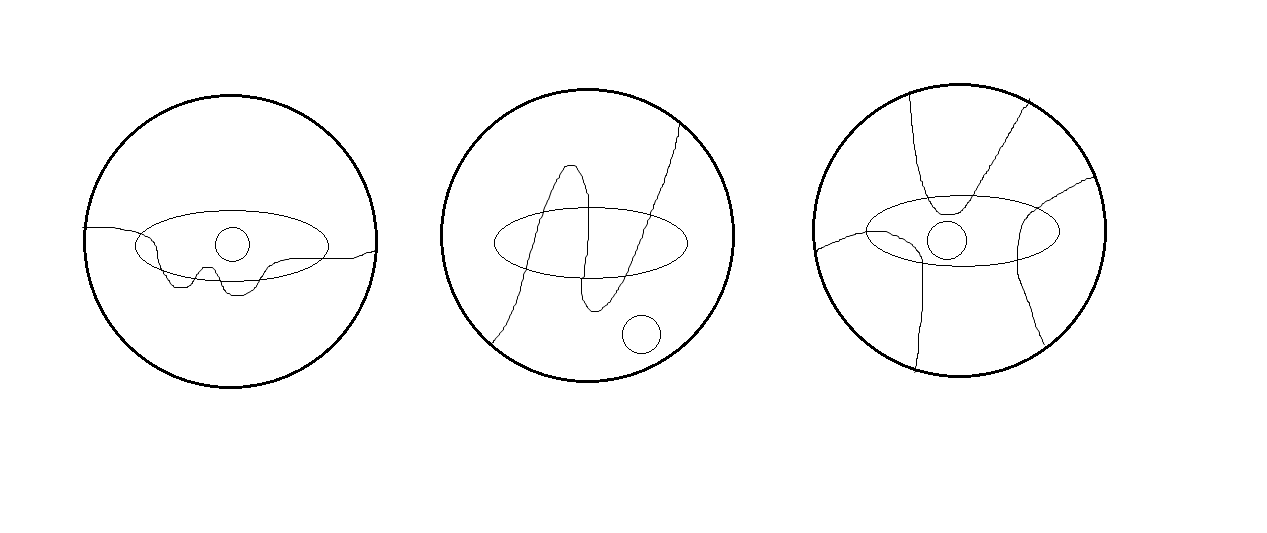
\includegraphics[scale=0.55]{ovals_and_loc_of_odd_brunch.png}}
\caption{Допустимые области для овалов}
\label{fig:ovals_and_loc_of_odd_brunch}
\end{figure}

Так как необходимо учитывать эти ограничения для каждой из двух коник, то для каждой ситуации (картинки) на рисунке \ref{fig:curves_without_ovals} надо найти пересечение допустимой области относительно одной коники с допустимой областью относительно второй коники.

\begin{figure}[H]
\center{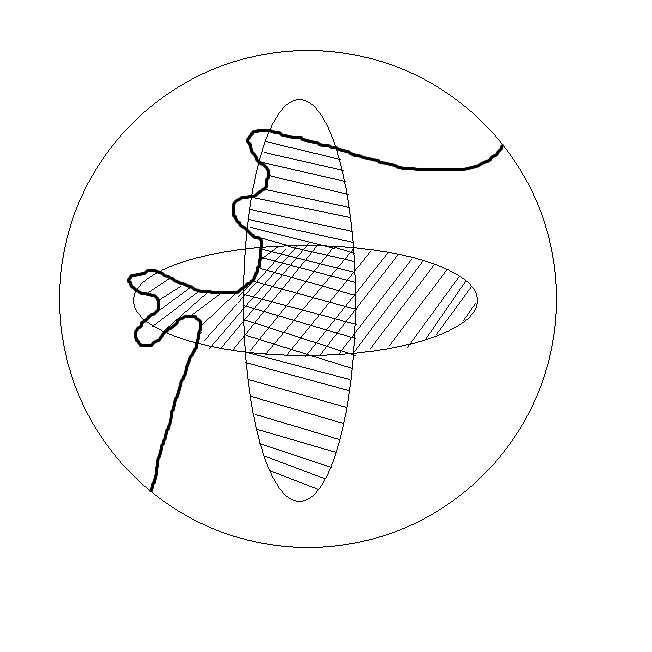
\includegraphics[scale=0.55]{intersection_of_fields.png}}
\caption{}
\label{fig:intersection_of_fields}
\end{figure}

Мы видим, что в некоторых случаях такие пересечения пустые, значит с данным расположением кривые рассматриваемого нами класса невозможны.

\begin{figure}[H]
\center{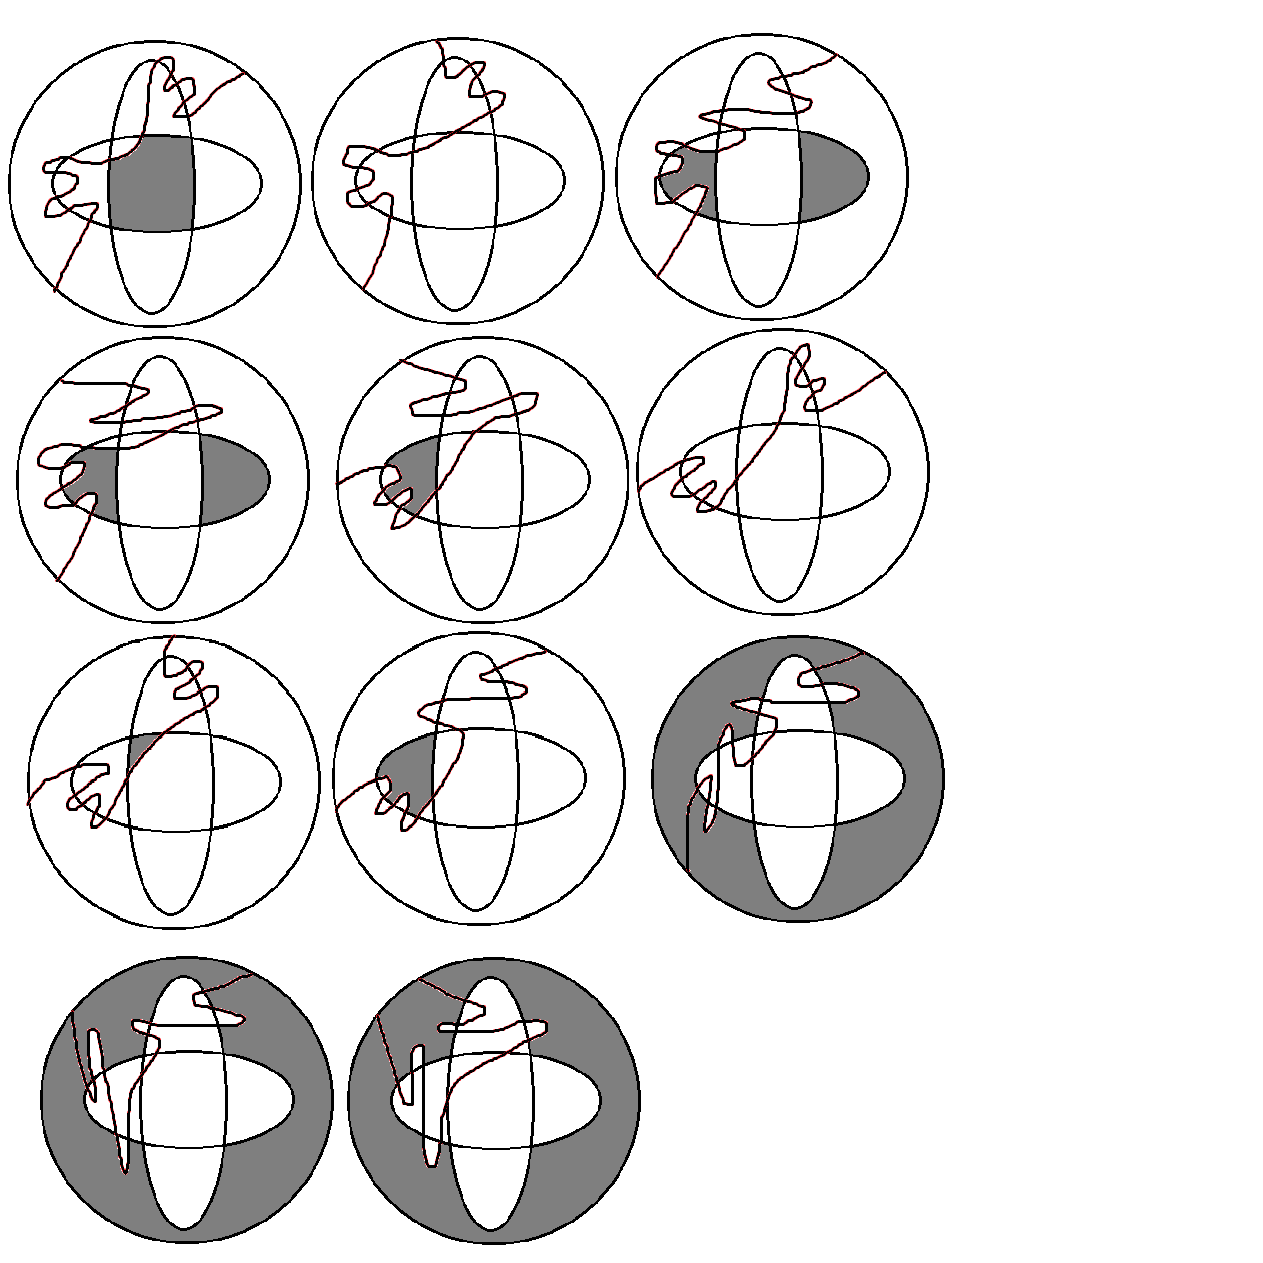
\includegraphics[scale=0.75]{curves_with_ovals.png}}
\caption{Модели с допустимыми областями для овала}
\label{fig:curves_with_ovals}
\end{figure}

Мы видим, что в некоторых случаях такие пересечения пустые, значит с данным расположением кривые рассматриваемого нами класса невозможны.
Заметим, что есть случаи, когда имеются по две области, допустимых для расположения в них овала.







%%\@input{preface}
%%\@input{ch1_1}
%%\@input{bibliography}
\makeatother
\end{document}
